\documentclass[aspectratio=169]{beamer}
\usetheme{metropolis}           % Use metropolis theme
\metroset{numbering=fraction}
\usepackage{tikz}
\usetikzlibrary{arrows,positioning,shapes.geometric}
\usepackage{float}
\usepackage{makecell}
\usepackage{fancyvrb}
\usepackage{listings}
\usepackage[export]{adjustbox}
\usepackage{caption}
\usepackage{alltt}
\title{Lecture 3 \\ More Java Basics \\ Interfaces and Abstract Classes}
\date{May 10, 2016}
\author{Patrick Lam \\ Jeff Zarnett \\ Michael Giannikouris}
\institute{Department of Electrical and Computer Engineering}
\setbeamertemplate{caption}{\raggedright\insertcaption\par}
\setbeamersize{text margin left=12pt,text margin right=12pt}
\newcommand{\putat}[3]{\begin{picture}(0,0)(0,0)\put(#1,#2){#3}\end{picture}} % just a shorthand

\newenvironment{deflist}
{ \begin{description}
    \setlength{\itemsep}{6pt}
    \setlength{\parskip}{0pt}
    \setlength{\parsep}{0pt}     }
{ \end{description}              } 

\newenvironment{splitslide}
{
\centering
\begin{tabular}{@{}p{0.50\textwidth} | p{0.025\textwidth}@{} p{0.4\textwidth}@{}}
}
{
\end{tabular}
}


\begin{document}
\maketitle



\section*{Java String Class}



%%%%%%%%%%%%%%%%%%%%%%%%%%%%%%%%%%%%%%%%%%%%%%%%%%%%%%%%%%%%%%%%%%%%%%%%%%%%%%%%%%%%
% Strings
%%%%%%%%%%%%%%%%%%%%%%%%%%%%%%%%%%%%%%%%%%%%%%%%%%%%%%%%%%%%%%%%%%%%%%%%%%%%%%%%%%%%
\begin{frame}{Strings}
\texttt{String} is a \textbf{class} (reference to a character array), \textbf{not} a primitive. \\
\vspace{0.5em}
\texttt{String} is \textbf{immutable}. Once created, a \texttt{String} cannot change. \\
\vspace{0.5em}
If you call a \texttt{String} method that modifies the string, a new \texttt{String} object is returned (the existing one does not change):\\
\vspace{1em}

\texttt{String string1 = "Hello World!";} \\
\texttt{String string2 = string1.replaceAll('?', '!')}, \\
\vspace{1em}

string1 still contains "Hello World!" \\
string2 contains "Hello World?"

\end{frame}
%%%%%%%%%%%%%%%%%%%%%%%%%%%%%%%%%%%%%%%%%%%%%%%%%%%%%%%%%%%%%%%%%%%%%%%%%%%%%%%%%%%%



%%%%%%%%%%%%%%%%%%%%%%%%%%%%%%%%%%%%%%%%%%%%%%%%%%%%%%%%%%%%%%%%%%%%%%%%%%%%%%%%%%%%
% Strings
%%%%%%%%%%%%%%%%%%%%%%%%%%%%%%%%%%%%%%%%%%%%%%%%%%%%%%%%%%%%%%%%%%%%%%%%%%%%%%%%%%%%
\begin{frame}{Strings and the == Operator}
The equality operator \texttt{==} can behave strangely when used on \texttt{String}. \\
\vspace{1em}
Use the \texttt{equals} method: \\
\texttt{if(string1.equals(string2)) \{ ... \} } \\
\vspace{1em}
This is an example of \textbf{reference equality} vs. \textbf{value equality}.
\end{frame}
%%%%%%%%%%%%%%%%%%%%%%%%%%%%%%%%%%%%%%%%%%%%%%%%%%%%%%%%%%%%%%%%%%%%%%%%%%%%%%%%%%%%



\section{Java Arrays}



%%%%%%%%%%%%%%%%%%%%%%%%%%%%%%%%%%%%%%%%%%%%%%%%%%%%%%%%%%%%%%%%%%%%%%%%%%%%%%%%%%%%
% Arrays and Collections
%%%%%%%%%%%%%%%%%%%%%%%%%%%%%%%%%%%%%%%%%%%%%%%%%%%%%%%%%%%%%%%%%%%%%%%%%%%%%%%%%%%%
\begin{frame}{Arrays \& Collections}
The simple array is created with the \texttt{[]} square brackets. \\
\vspace{0.5em}
Example: \texttt{int[] numbers = new int[10];} \\

\begin{center}
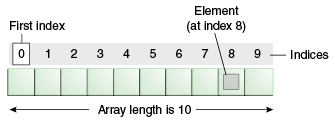
\includegraphics[height=0.35\textheight]{img/objects-tenElementArray.png}
\footnote{https://docs.oracle.com/javase/tutorial/java/nutsandbolts/arrays.html}
\end{center}

You can have null elements in an array (say, of Strings) without affecting the array length. \\
\vspace{0.5em}
An array is technically an object, so you can assign it where any \texttt{Object} is expected. \\
\vspace{2em}
\end{frame}
%%%%%%%%%%%%%%%%%%%%%%%%%%%%%%%%%%%%%%%%%%%%%%%%%%%%%%%%%%%%%%%%%%%%%%%%%%%%%%%%%%%%



%%%%%%%%%%%%%%%%%%%%%%%%%%%%%%%%%%%%%%%%%%%%%%%%%%%%%%%%%%%%%%%%%%%%%%%%%%%%%%%%%%%%
% Arrays
%%%%%%%%%%%%%%%%%%%%%%%%%%%%%%%%%%%%%%%%%%%%%%%%%%%%%%%%%%%%%%%%%%%%%%%%%%%%%%%%%%%%
\begin{frame}{Arrays}
Multidimensional arrays are also allowed, but only for primitive types \\
\vspace{1em}
\texttt{int[][][]  coordinates = new int[5][10][2];}.  \\
\vspace{1em}
This is not a big restriction since you can just have an array of arrays. \\
\vspace{1em}
Unlike some languages (C\#), you can't specify a rectangular array. \\
\end{frame}
%%%%%%%%%%%%%%%%%%%%%%%%%%%%%%%%%%%%%%%%%%%%%%%%%%%%%%%%%%%%%%%%%%%%%%%%%%%%%%%%%%%%



%%%%%%%%%%%%%%%%%%%%%%%%%%%%%%%%%%%%%%%%%%%%%%%%%%%%%%%%%%%%%%%%%%%%%%%%%%%%%%%%%%%%
% Arrays
%%%%%%%%%%%%%%%%%%%%%%%%%%%%%%%%%%%%%%%%%%%%%%%%%%%%%%%%%%%%%%%%%%%%%%%%%%%%%%%%%%%%
\begin{frame}{Arrays}
Arrays are great, but like \texttt{String} an explicit array has a fixed size. \\
\vspace{2em}
What if we don't know how many element we need at compile time? \\
\begin{itemize}
\item Create a new, bigger array and copy all the data?  \\
\item Allocate a very large array (i.e. 1000 elements) upfront? \\
\end{itemize}
\vspace{2em}
Wouldn't it be nice if we had a \textbf{dynamic} collection? \\
\end{frame}
%%%%%%%%%%%%%%%%%%%%%%%%%%%%%%%%%%%%%%%%%%%%%%%%%%%%%%%%%%%%%%%%%%%%%%%%%%%%%%%%%%%%



\section*{Java Collections}



%%%%%%%%%%%%%%%%%%%%%%%%%%%%%%%%%%%%%%%%%%%%%%%%%%%%%%%%%%%%%%%%%%%%%%%%%%%%%%%%%%%%
% Java Collections
%%%%%%%%%%%%%%%%%%%%%%%%%%%%%%%%%%%%%%%%%%%%%%%%%%%%%%%%%%%%%%%%%%%%%%%%%%%%%%%%%%%%
\begin{frame}{Java Collections}
In Java, we do, and they're called, \texttt{Collection}s. \\
\vspace{1em}
The most common one: the \texttt{List}.  \\
\vspace{1em}
The size of a \texttt{List} can change dynamically...how this is done is dependent on the type of List. \\
\end{frame}
%%%%%%%%%%%%%%%%%%%%%%%%%%%%%%%%%%%%%%%%%%%%%%%%%%%%%%%%%%%%%%%%%%%%%%%%%%%%%%%%%%%%



%%%%%%%%%%%%%%%%%%%%%%%%%%%%%%%%%%%%%%%%%%%%%%%%%%%%%%%%%%%%%%%%%%%%%%%%%%%%%%%%%%%%
% Lists
%%%%%%%%%%%%%%%%%%%%%%%%%%%%%%%%%%%%%%%%%%%%%%%%%%%%%%%%%%%%%%%%%%%%%%%%%%%%%%%%%%%%
\begin{frame}{Lists}
There are many kinds of \texttt{List} implementations in Java. There is no plain \texttt{List} class that you can instantiate. \\
\vspace{1em}
Be specific about what kind of list you want to have, such as \texttt{ArrayList} (a very common one) or \texttt{LinkedList}. \\
\vspace{1em}
A List takes a parameter in angle brackets to tell you what it is a list of. \\
\vspace{1em}
Example: \texttt{ArrayList<String> myList = new ArrayList<String>();}
\end{frame}
%%%%%%%%%%%%%%%%%%%%%%%%%%%%%%%%%%%%%%%%%%%%%%%%%%%%%%%%%%%%%%%%%%%%%%%%%%%%%%%%%%%%



%%%%%%%%%%%%%%%%%%%%%%%%%%%%%%%%%%%%%%%%%%%%%%%%%%%%%%%%%%%%%%%%%%%%%%%%%%%%%%%%%%%%
% Three Basic Collections
%%%%%%%%%%%%%%%%%%%%%%%%%%%%%%%%%%%%%%%%%%%%%%%%%%%%%%%%%%%%%%%%%%%%%%%%%%%%%%%%%%%%
\begin{frame}{Three Basic Collections}
Three basic collections exist: \\
\vspace{0.5em}
\begin{enumerate}
	\item List
	\item Map (in a later lecture)
	\item Set (like a list, but no duplicates)
\end{enumerate}
\end{frame}
%%%%%%%%%%%%%%%%%%%%%%%%%%%%%%%%%%%%%%%%%%%%%%%%%%%%%%%%%%%%%%%%%%%%%%%%%%%%%%%%%%%%


\section*{More Java Keywords}


%%%%%%%%%%%%%%%%%%%%%%%%%%%%%%%%%%%%%%%%%%%%%%%%%%%%%%%%%%%%%%%%%%%%%%%%%%%%%%%%%%%%
% static
%%%%%%%%%%%%%%%%%%%%%%%%%%%%%%%%%%%%%%%%%%%%%%%%%%%%%%%%%%%%%%%%%%%%%%%%%%%%%%%%%%%%
\begin{frame}{\texttt{static}}
When you see something with the keyword \texttt{static}, it means there is only one copy. \\
\vspace{2em}
Let's see how this works in relation to fields, methods, and classes.
\end{frame}
%%%%%%%%%%%%%%%%%%%%%%%%%%%%%%%%%%%%%%%%%%%%%%%%%%%%%%%%%%%%%%%%%%%%%%%%%%%%%%%%%%%%



%%%%%%%%%%%%%%%%%%%%%%%%%%%%%%%%%%%%%%%%%%%%%%%%%%%%%%%%%%%%%%%%%%%%%%%%%%%%%%%%%%%%
% Static Variable
%%%%%%%%%%%%%%%%%%%%%%%%%%%%%%%%%%%%%%%%%%%%%%%%%%%%%%%%%%%%%%%%%%%%%%%%%%%%%%%%%%%%
\begin{frame}{Static Variable}
\begin{columns}
\begin{column}{0.05\textwidth}
\end{column}
\begin{column}{0.35\textwidth}
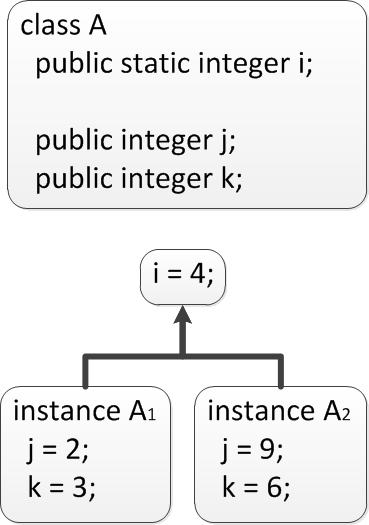
\includegraphics[height=0.8\textheight]{img/A1A2.png}
\end{column}
\begin{column}{0.55\textwidth}
A static variable is common to all instances of the class. \\
\vspace{1em}
Assume class $A$ has integer \texttt{i}, and there are two class instances called $A_{1}$ and $A_{2}$. \\
\vspace{1em}
The value of \texttt{i} is the same and shared between objects $A_{1}$ and $A_{2}$. \\
\end{column}
\begin{column}{0.05\textwidth}
\end{column}
\end{columns}
\end{frame}
%%%%%%%%%%%%%%%%%%%%%%%%%%%%%%%%%%%%%%%%%%%%%%%%%%%%%%%%%%%%%%%%%%%%%%%%%%%%%%%%%%%%



%%%%%%%%%%%%%%%%%%%%%%%%%%%%%%%%%%%%%%%%%%%%%%%%%%%%%%%%%%%%%%%%%%%%%%%%%%%%%%%%%%%%
% Static Method
%%%%%%%%%%%%%%%%%%%%%%%%%%%%%%%%%%%%%%%%%%%%%%%%%%%%%%%%%%%%%%%%%%%%%%%%%%%%%%%%%%%%
\begin{frame}{Static Method}
The method is shared between all instances of the class. 	\\
\vspace{1em}
Static method cannot access instance variables/methods of the class...		\\
\quad\quad ...only methods and variables that share the static modifier. \\
\vspace{1em}
For example, \texttt{main()} in Java is declared as \texttt{static} (a program has one main())... \\
\quad ...declare variables as \texttt{static} to reference them in \texttt{main}. \\
\vspace{1em}
A Java static method cannot be overridden in a subclass.
\end{frame}
%%%%%%%%%%%%%%%%%%%%%%%%%%%%%%%%%%%%%%%%%%%%%%%%%%%%%%%%%%%%%%%%%%%%%%%%%%%%%%%%%%%%



%%%%%%%%%%%%%%%%%%%%%%%%%%%%%%%%%%%%%%%%%%%%%%%%%%%%%%%%%%%%%%%%%%%%%%%%%%%%%%%%%%%%
% Static Class
%%%%%%%%%%%%%%%%%%%%%%%%%%%%%%%%%%%%%%%%%%%%%%%%%%%%%%%%%%%%%%%%%%%%%%%%%%%%%%%%%%%%
\begin{frame}{Static Class}
The static modifier cannot be applied to a class. \\
\vspace{2em}
However, we will see that some classes are composed entirely of static components. \\
\end{frame}
%%%%%%%%%%%%%%%%%%%%%%%%%%%%%%%%%%%%%%%%%%%%%%%%%%%%%%%%%%%%%%%%%%%%%%%%%%%%%%%%%%%%



%%%%%%%%%%%%%%%%%%%%%%%%%%%%%%%%%%%%%%%%%%%%%%%%%%%%%%%%%%%%%%%%%%%%%%%%%%%%%%%%%%%%
% final
%%%%%%%%%%%%%%%%%%%%%%%%%%%%%%%%%%%%%%%%%%%%%%%%%%%%%%%%%%%%%%%%%%%%%%%%%%%%%%%%%%%%
\begin{frame}{\texttt{final}}
Another keyword: \texttt{final}. This can be applied to three things, with slightly different meanings:
\begin{description}
	\item[Field] We field value is constant
	\item[Method] The method cannot be overridden
	\item[Class] The class cannot be subclassed
\end{description}
\end{frame}
%%%%%%%%%%%%%%%%%%%%%%%%%%%%%%%%%%%%%%%%%%%%%%%%%%%%%%%%%%%%%%%%%%%%%%%%%%%%%%%%%%%%



\section*{Java's Math Class}



%%%%%%%%%%%%%%%%%%%%%%%%%%%%%%%%%%%%%%%%%%%%%%%%%%%%%%%%%%%%%%%%%%%%%%%%%%%%%%%%%%%%
% Java's Math Class
%%%%%%%%%%%%%%%%%%%%%%%%%%%%%%%%%%%%%%%%%%%%%%%%%%%%%%%%%%%%%%%%%%%%%%%%%%%%%%%%%%%%
\begin{frame}[fragile]{Java's Math Class}
\begin{splitslide}

\begin{Verbatim}[fontsize=\tiny]
public final class Math {
  private Math() {}
  
  public static final double E = 2.7182818284590452354;
  
  public static final double PI = 3.14159265358979323846;
  
  public static double sin(double a) {
    // returns sine  
  }
  
  public static double cos(double a) {
    // returns cos  
  }
  
  .
  .
  .
}
\end{Verbatim}

&&

\raggedright
\vspace{1em}
The Math class in Java nicely demonstrates the \texttt{static} and \texttt{final} keywords. \\
\vspace{1em}
The Math class is a collection of mathematical functions (e.g. trigonometry) and a some constants (e.g. pi). \\

\end{splitslide}
\end{frame}
%%%%%%%%%%%%%%%%%%%%%%%%%%%%%%%%%%%%%%%%%%%%%%%%%%%%%%%%%%%%%%%%%%%%%%%%%%%%%%%%%%%%



%%%%%%%%%%%%%%%%%%%%%%%%%%%%%%%%%%%%%%%%%%%%%%%%%%%%%%%%%%%%%%%%%%%%%%%%%%%%%%%%%%%%
% Java's Math Class
%%%%%%%%%%%%%%%%%%%%%%%%%%%%%%%%%%%%%%%%%%%%%%%%%%%%%%%%%%%%%%%%%%%%%%%%%%%%%%%%%%%%
\begin{frame}[fragile]{Java's Math Class}
\begin{splitslide}

\begin{Verbatim}[fontsize=\tiny]
public final class Math {
  private Math() {}
  
  public static final double E = 2.7182818284590452354;
  
  public static final double PI = 3.14159265358979323846;
  
  public static double sin(double a) {
    // returns sine  
  }
  
  public static double cos(double a) {
    // returns cos  
  }
  
  .
  .
  .
}
\end{Verbatim}

&&

\raggedright
\vspace{1em}
\begin{footnotesize}
We don't need to incur the overhead of instantiating a class just to, say, take a cosine. There is no state (fields), and no reason to have instances of the class. \\
\vspace{0.5em}
So, Math class methods are \texttt{static}; we call them without an instance of the class. \\
\vspace{0.5em}
The Math class is also \texttt{final}, we cannot subclass it.
\end{footnotesize}

\end{splitslide}
\end{frame}
%%%%%%%%%%%%%%%%%%%%%%%%%%%%%%%%%%%%%%%%%%%%%%%%%%%%%%%%%%%%%%%%%%%%%%%%%%%%%%%%%%%%



%%%%%%%%%%%%%%%%%%%%%%%%%%%%%%%%%%%%%%%%%%%%%%%%%%%%%%%%%%%%%%%%%%%%%%%%%%%%%%%%%%%%
% Java's Math Class
%%%%%%%%%%%%%%%%%%%%%%%%%%%%%%%%%%%%%%%%%%%%%%%%%%%%%%%%%%%%%%%%%%%%%%%%%%%%%%%%%%%%
\begin{frame}[fragile]{Java's Math Class}
\begin{splitslide}

\begin{Verbatim}[fontsize=\tiny]
public final class Math {
  private Math() {}
  
  public static final double E = 2.7182818284590452354;
  
  public static final double PI = 3.14159265358979323846;
  
  public static double sin(double a) {
    // returns sine  
  }
  
  public static double cos(double a) {
    // returns cos  
  }
  
  .
  .
  .
}
\end{Verbatim}

&&

\raggedright
\vspace{1em}
The Math class demonstrates something else interesting: \textbf{private constructors}. \\
\vspace{0.5em}
A private constructor, as the access modifier suggests, cannot be called from outside the class. \\
\vspace{0.5em}
The effect is that, if we have \textbf{only} a \texttt{private} constructor, we cannot instantiate the class! \\

\end{splitslide}
\end{frame}
%%%%%%%%%%%%%%%%%%%%%%%%%%%%%%%%%%%%%%%%%%%%%%%%%%%%%%%%%%%%%%%%%%%%%%%%%%%%%%%%%%%%



\section*{Java Review}



\begin{frame}{Java Review}
Let's spend a little bit of time in a Java environment to consolidate our Java knowledge.
\end{frame}

\section*{Java Interfaces}



%%%%%%%%%%%%%%%%%%%%%%%%%%%%%%%%%%%%%%%%%%%%%%%%%%%%%%%%%%%%%%%%%%%%%%%%%%%%%%%%%%%%
% Interfaces
%%%%%%%%%%%%%%%%%%%%%%%%%%%%%%%%%%%%%%%%%%%%%%%%%%%%%%%%%%%%%%%%%%%%%%%%%%%%%%%%%%%%
\begin{frame}{Interfaces}
\only<1>{One of these things is not like the others:}
\only<2>{All but one of these things implements the {\tt HasHandle} interface.}
\begin{center}
\begin{tabular}{l l l l}
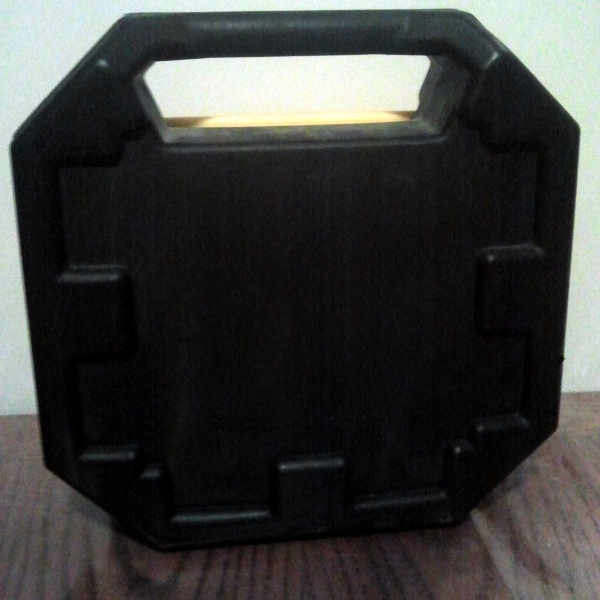
\includegraphics[width=.22\textwidth]{img/box-scaled.jpg} &
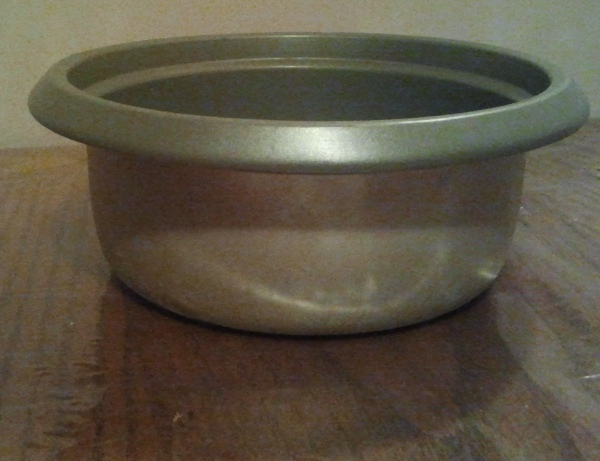
\includegraphics[width=.22\textwidth]{img/bowl-scaled.jpg} &
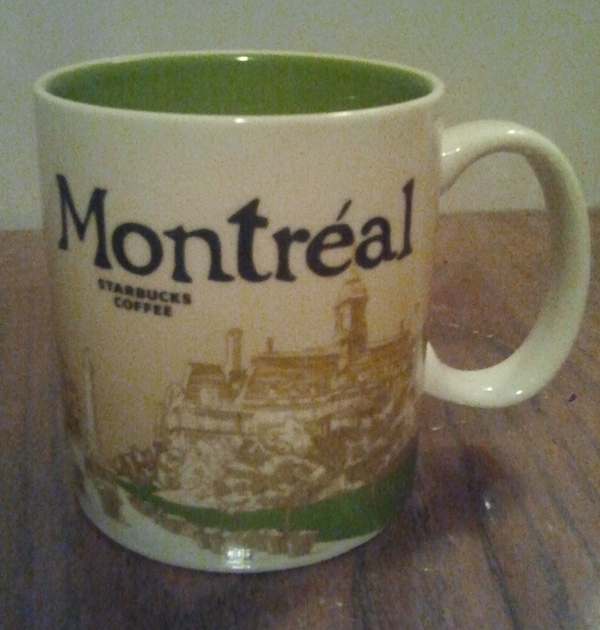
\includegraphics[width=.22\textwidth]{img/mug-scaled} &
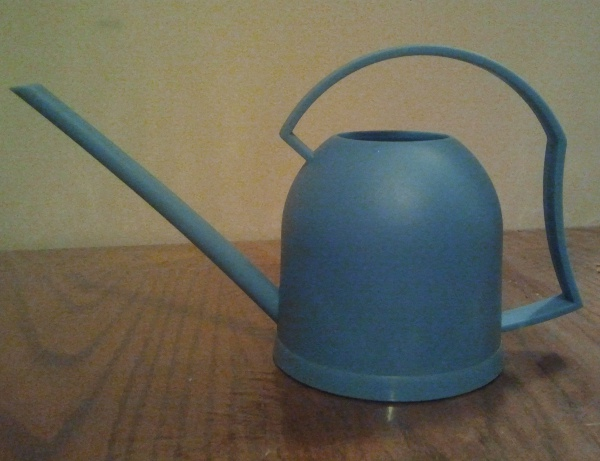
\includegraphics[width=.22\textwidth]{img/wateringcan-scaled.jpg} \\
\end{tabular}
\end{center}
\end{frame}
%%%%%%%%%%%%%%%%%%%%%%%%%%%%%%%%%%%%%%%%%%%%%%%%%%%%%%%%%%%%%%%%%%%%%%%%%%%%%%%%%%%%



%%%%%%%%%%%%%%%%%%%%%%%%%%%%%%%%%%%%%%%%%%%%%%%%%%%%%%%%%%%%%%%%%%%%%%%%%%%%%%%%%%%%
% Interfaces as Contracts
%%%%%%%%%%%%%%%%%%%%%%%%%%%%%%%%%%%%%%%%%%%%%%%%%%%%%%%%%%%%%%%%%%%%%%%%%%%%%%%%%%%%
\begin{frame}{Interfaces as Contracts}
An \texttt{interface} is a way of specifying in Java what is effectively a contract. \\
\vspace{1em}
The interface specifies some number of methods which any class that wants to implement this interface must have. \\
\vspace{1em}
The \textbf{implementation} of these methods up to the classes that \alert{implement} the interface. 
\end{frame}
%%%%%%%%%%%%%%%%%%%%%%%%%%%%%%%%%%%%%%%%%%%%%%%%%%%%%%%%%%%%%%%%%%%%%%%%%%%%%%%%%%%%



%%%%%%%%%%%%%%%%%%%%%%%%%%%%%%%%%%%%%%%%%%%%%%%%%%%%%%%%%%%%%%%%%%%%%%%%%%%%%%%%%%%%
% Using Interfaces
%%%%%%%%%%%%%%%%%%%%%%%%%%%%%%%%%%%%%%%%%%%%%%%%%%%%%%%%%%%%%%%%%%%%%%%%%%%%%%%%%%%%
\begin{frame}{Using Interfaces}
\begin{alltt}
  interface HasHandle \{ \\
\qquad    void pickup(); \\
  \}\\[1em]
  class WateringCan \alert{implements} HasHandle \{ \\
\qquad    void pickup() \{ \ldots~\}  \\
\qquad    \ldots \\
  \}\\
\end{alltt}
\vspace{0.5em}
Interfaces do not contain implementation (there is one exception).\\
\vspace{1em}
A class which implements \texttt{HasHandle} \textbf{must} provide an implementation of \texttt{pickup()}.
\end{frame}
%%%%%%%%%%%%%%%%%%%%%%%%%%%%%%%%%%%%%%%%%%%%%%%%%%%%%%%%%%%%%%%%%%%%%%%%%%%%%%%%%%%%



%%%%%%%%%%%%%%%%%%%%%%%%%%%%%%%%%%%%%%%%%%%%%%%%%%%%%%%%%%%%%%%%%%%%%%%%%%%%%%%%%%%%
% Interfaces Semantics
%%%%%%%%%%%%%%%%%%%%%%%%%%%%%%%%%%%%%%%%%%%%%%%%%%%%%%%%%%%%%%%%%%%%%%%%%%%%%%%%%%%%
\begin{frame}{Interface Semantics}
Methods that are declared in an interface are always \texttt{public}. \\
\vspace{0.5em}
Interfaces can extend other (and multiple) interfaces. \\
\vspace{0.5em}
An interface may declare some constant fields. \\
\vspace{0.5em}
An interface can never be instantiated. \\
\vspace{0.5em}
A class can implement as many interfaces as desired. \\
\vspace{0.5em}
We cannot apply the \texttt{final} keyword to an interface class, because we obviously have to implement it somehow.
\end{frame}
%%%%%%%%%%%%%%%%%%%%%%%%%%%%%%%%%%%%%%%%%%%%%%%%%%%%%%%%%%%%%%%%%%%%%%%%%%%%%%%%%%%%



%%%%%%%%%%%%%%%%%%%%%%%%%%%%%%%%%%%%%%%%%%%%%%%%%%%%%%%%%%%%%%%%%%%%%%%%%%%%%%%%%%%%
% Why Interfaces?
%%%%%%%%%%%%%%%%%%%%%%%%%%%%%%%%%%%%%%%%%%%%%%%%%%%%%%%%%%%%%%%%%%%%%%%%%%%%%%%%%%%%
\begin{frame}{Why Interfaces?}
Interact with an object without knowing specifics about it. \\
\vspace{1em}
Interact with many different objects in a uniform way. \\
\vspace{1em}
Example: \texttt{Comparable} allows the JRE to sort objects. \\
\vspace{1em}
For a built-in sort, the object must implement \texttt{Comparable}.\\ \quad (otherwise Java has no idea how to order them). \\
\vspace{1em}
\texttt{Comparable}: only one method (\texttt{CompareTo}) is required.
\end{frame}
%%%%%%%%%%%%%%%%%%%%%%%%%%%%%%%%%%%%%%%%%%%%%%%%%%%%%%%%%%%%%%%%%%%%%%%%%%%%%%%%%%%%



\section*{Java Abstract Classes}



%%%%%%%%%%%%%%%%%%%%%%%%%%%%%%%%%%%%%%%%%%%%%%%%%%%%%%%%%%%%%%%%%%%%%%%%%%%%%%%%%%%%
% Abstract Classes
%%%%%%%%%%%%%%%%%%%%%%%%%%%%%%%%%%%%%%%%%%%%%%%%%%%%%%%%%%%%%%%%%%%%%%%%%%%%%%%%%%%%
\begin{frame}{Abstract Classes}
Halfway between an interface and a regular class is the \alert{abstract class}.

May (but does not have to) contain abstract methods. 

Any class that contains methods marked \texttt{abstract} must also be marked as \texttt{abstract}. 

Cannot be instantiated, but may be subclassed. 

We cannot apply the \texttt{final} keyword to an abstract class, because it's meant to be subclassed.

An abstract class can have as much or as little implementation as desired.
\end{frame}
%%%%%%%%%%%%%%%%%%%%%%%%%%%%%%%%%%%%%%%%%%%%%%%%%%%%%%%%%%%%%%%%%%%%%%%%%%%%%%%%%%%%



%%%%%%%%%%%%%%%%%%%%%%%%%%%%%%%%%%%%%%%%%%%%%%%%%%%%%%%%%%%%%%%%%%%%%%%%%%%%%%%%%%%%
% Abstract Classes
%%%%%%%%%%%%%%%%%%%%%%%%%%%%%%%%%%%%%%%%%%%%%%%%%%%%%%%%%%%%%%%%%%%%%%%%%%%%%%%%%%%%
\begin{frame}[fragile]{Abstract Classes}
To declare an abstract method, write the method signature, but with the keyword \texttt{abstract} attached: \\
\vspace{2em}
\verb+public abstract void draw(int parameter);+\\
\vspace{2em}
Abstract classes may have static fields and methods.\\
\quad e.g. \texttt{AbstractClass.method()}.
\end{frame}
%%%%%%%%%%%%%%%%%%%%%%%%%%%%%%%%%%%%%%%%%%%%%%%%%%%%%%%%%%%%%%%%%%%%%%%%%%%%%%%%%%%%



%%%%%%%%%%%%%%%%%%%%%%%%%%%%%%%%%%%%%%%%%%%%%%%%%%%%%%%%%%%%%%%%%%%%%%%%%%%%%%%%%%%%
% Abstract Classes vs. Interfaces
%%%%%%%%%%%%%%%%%%%%%%%%%%%%%%%%%%%%%%%%%%%%%%%%%%%%%%%%%%%%%%%%%%%%%%%%%%%%%%%%%%%%
\begin{frame}{Abstract Classes vs. Interfaces}
There are similarities between abstract classes \& interfaces. \\
\vspace{1em}
When should each of these be used?
\end{frame}
%%%%%%%%%%%%%%%%%%%%%%%%%%%%%%%%%%%%%%%%%%%%%%%%%%%%%%%%%%%%%%%%%%%%%%%%%%%%%%%%%%%%



%%%%%%%%%%%%%%%%%%%%%%%%%%%%%%%%%%%%%%%%%%%%%%%%%%%%%%%%%%%%%%%%%%%%%%%%%%%%%%%%%%%%
% Use Abstract Class When
%%%%%%%%%%%%%%%%%%%%%%%%%%%%%%%%%%%%%%%%%%%%%%%%%%%%%%%%%%%%%%%%%%%%%%%%%%%%%%%%%%%%
\begin{frame}{Use Abstract Class When}
\begin{itemize}
\item To share code among several closely related classes.
\item Classes that extend your abstract class have many common methods or fields, or require access modifiers other than public (such as protected and private).
\item To declare non-static or non-final fields. 
\end{itemize}
\end{frame}
%%%%%%%%%%%%%%%%%%%%%%%%%%%%%%%%%%%%%%%%%%%%%%%%%%%%%%%%%%%%%%%%%%%%%%%%%%%%%%%%%%%%



%%%%%%%%%%%%%%%%%%%%%%%%%%%%%%%%%%%%%%%%%%%%%%%%%%%%%%%%%%%%%%%%%%%%%%%%%%%%%%%%%%%%
% Use Interface When
%%%%%%%%%%%%%%%%%%%%%%%%%%%%%%%%%%%%%%%%%%%%%%%%%%%%%%%%%%%%%%%%%%%%%%%%%%%%%%%%%%%%
\begin{frame}{Use Interface When}
\begin{itemize}
\item Unrelated classes would implement your interface. 
\item You want to specify the behaviour of a particular data type, but not concerned about who implements its behaviour.
\item You want to take advantage of multiple inheritance of type (i.e. implement multiple interfaces on one class)
\end{itemize}
\end{frame}
%%%%%%%%%%%%%%%%%%%%%%%%%%%%%%%%%%%%%%%%%%%%%%%%%%%%%%%%%%%%%%%%%%%%%%%%%%%%%%%%%%%%



%%%%%%%%%%%%%%%%%%%%%%%%%%%%%%%%%%%%%%%%%%%%%%%%%%%%%%%%%%%%%%%%%%%%%%%%%%%%%%%%%%%%
% Why Not Both?
%%%%%%%%%%%%%%%%%%%%%%%%%%%%%%%%%%%%%%%%%%%%%%%%%%%%%%%%%%%%%%%%%%%%%%%%%%%%%%%%%%%%
\begin{frame}{Why Not Both?}
An interface can be partly implemented by an abstract class. \\
\vspace{1em}
The concrete class that extends the abstract class is responsible for implementing any of the methods of the interface that its superclass does not. \\
\end{frame}
%%%%%%%%%%%%%%%%%%%%%%%%%%%%%%%%%%%%%%%%%%%%%%%%%%%%%%%%%%%%%%%%%%%%%%%%%%%%%%%%%%%%



%%%%%%%%%%%%%%%%%%%%%%%%%%%%%%%%%%%%%%%%%%%%%%%%%%%%%%%%%%%%%%%%%%%%%%%%%%%%%%%%%%%%
% Why Not Both?
%%%%%%%%%%%%%%%%%%%%%%%%%%%%%%%%%%%%%%%%%%%%%%%%%%%%%%%%%%%%%%%%%%%%%%%%%%%%%%%%%%%%
\begin{frame}{Why Not Both?}
\begin{center}
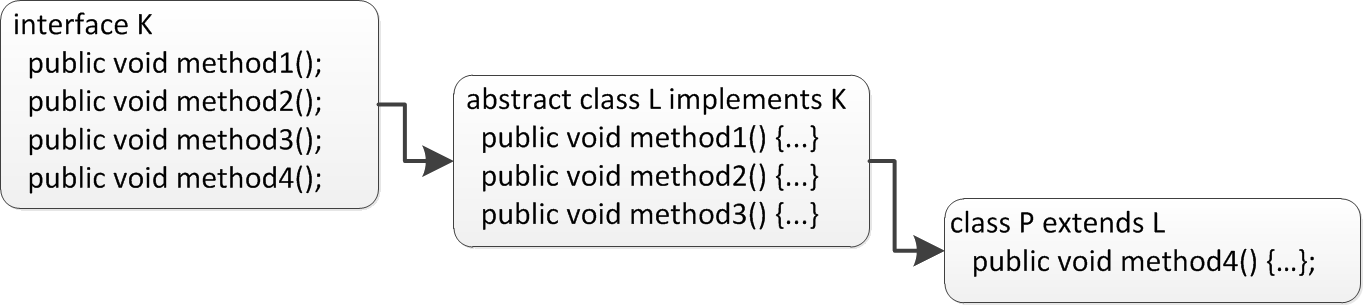
\includegraphics[width=0.95\textwidth]{img/KLP.png} 
\end{center}

\vspace{1em}
When a subclass $P$ of $L$ is declared, then $P$ must implement that method that $L$ did not (or else be abstract itself). \\
\end{frame}
%%%%%%%%%%%%%%%%%%%%%%%%%%%%%%%%%%%%%%%%%%%%%%%%%%%%%%%%%%%%%%%%%%%%%%%%%%%%%%%%%%%%


\end{document}